% dodałem pakiet verbatim
\documentclass[b5paper,10pt,twoside]{book}
\usepackage[table]{xcolor}
\definecolor{lightgray}{gray}{0.9}
\usepackage[T1]{fontenc}
\usepackage{emptypage}
\usepackage[polish]{babel}
\usepackage[utf8]{inputenc}
\usepackage{etoolbox}
\usepackage{lmodern}
\usepackage{indentfirst} 
\usepackage{fancyhdr}
\usepackage{xcolor}
\usepackage{etoolbox} 
\usepackage{tocloft}
\usepackage{graphicx}
\usepackage{epstopdf}
\usepackage{geometry}
\usepackage{makeidx}
\usepackage{tabularx}
\usepackage[font=footnotesize ,labelfont=bf]{caption}
\usepackage[hang,flushmargin]{footmisc}
\usepackage{booktabs}
\usepackage{multirow}
\usepackage{mathtools}
\usepackage{apacite}
\usepackage{natbib}
\usepackage[hidelinks]{hyperref}
\setlength{\footnotesep}{0pt}
\setlength{\skip\footins}{0pt}
\renewcommand\footnoterule{\vspace*{7pt}\hrule width 2.5cm\vspace*{4.6pt}}
\let\lll\undefined
\usepackage{amssymb}
\usepackage{tabularx}
\newcolumntype{S}{@{\stepcounter{Definition}~} >{\bfseries}l @{~--~}X@{}}
\newcounter{Definition}[subsection]
% wyśrodkowanie komórek w tabelkach: \renewcommand{\tabularxcolumn}[1]{>{\small}m{#1}}
\renewcommand{\labelitemi}{\scriptsize$\square$   }
\setlength{\footnotemargin}{3mm}
%\newgeometry{bottom=1.5in, top=1.4in, footskip=0.7in, headsep=0.43in}
\geometry{papersize={170.4mm,243mm}, bottom=2.02795cm, top=2.02795cm, footskip=0.7cm, headsep=0.3527778cm, left=1.5cm, right=1.5cm, textheight=576.00pt}
\selectlanguage{polish}
\pagestyle{fancy}
\fancyhf{}
\renewcommand{\headrulewidth}{0pt}
\renewcommand{\footrulewidth}{0pt}
\renewcommand{\arraystretch}{1.4}\addtolength{\tabcolsep}{-1pt}
\fancyhead{} % clear all fields
\fancyfoot{} % clear all fields
\fancyhead[LE]{Księga wizualizacji składu książki}
\fancyhead[RO]{\nouppercase{\leftmark}}
\fancyfoot[LE,RO]{\thepage}
\makeatletter
\patchcmd{\@fancyhead}{\rlap}{\color{darkgray}\rlap}{}{}
\patchcmd{\headrule}{\hrule}{\color{darkgray}\hrule}{}{}
\makeatother
\widowpenalty=10000
\clubpenalty=10000
\usepackage{lettrine}\sloppy %zakaz wydłużania lini (gdzy nie może złożyć)
\fancypagestyle{plain}{%
   	\fancyhf{}                          % clear all header and footer fields
    \renewcommand{\headrulewidth}{0pt}
	\renewcommand{\footrulewidth}{0pt}
	\fancyfoot[LE,RO]{\thepage}
}
\graphicspath{ {Obrazy/} }
\makeindex
\usepackage[cam,a4,center]{crop}
\parskip 0pt
\usepackage[compact]{titlesec}
\titlespacing{\section}{0pt}{30pt}{15.6pt}
\titlespacing{\subsection}{0pt}{24pt}{12pt}
\titlespacing{\subsubsection}{0pt}{18pt}{8pt}
\titlespacing{\paragraph}{15pt}{2pt}{6pt}
\usepackage{enumitem}
\setlist{nolistsep}
\setlist[itemize]{topsep=0pt}
\renewcommand{\abovecaptionskip}{12pt}
\renewcommand{\belowcaptionskip}{0pt}
\renewcommand{\textfloatsep}{12pt}
\makeatletter
\newcommand\thefontsize{The current font size is: \f@size pt}
\makeatother
\makeatletter
\def\@makechapterhead#1{%
  %%%%\vspace*{50\p@}% %%% removed!
  {\parindent \z@ \raggedright \normalfont
    \ifnum \c@secnumdepth >\m@ne
        \huge\bfseries \@chapapp\space \thechapter
        \par\nobreak
        \vskip 15.2\p@
    \fi
    \interlinepenalty\@M
    \Huge \bfseries #1\par\nobreak
    \vskip 36\p@
  }}
\def\@makeschapterhead#1{%
  %%%%%\vspace*{50\p@}% %%% removed!
  {\parindent \z@ \raggedright
    \normalfont
    \interlinepenalty\@M
    \Huge \bfseries  #1\par\nobreak
    \vskip 36\p@
  }}
\newcommand{\customchapter}[2]{
    \setcounter{chapter}{#1}
    \setcounter{section}{0}
    \chapter*{#2}
    \addcontentsline{toc}{chapter}{#2}
}
\newcommand{\customtitle}[2]{
	\begin{flushleft}\textbf{#1 } #2 \end{flushleft}
	\par\medskip
	\rowcolors{1}{}{lightgray}
}
\makeatother



 \begin{comment}
\begin{knitrout}
\definecolor{shadecolor}{rgb}{0.969, 0.969, 0.969}\color{fgcolor}\begin{kframe}


{\ttfamily\noindent\itshape\color{messagecolor}{\#\# KernSmooth 2.23 loaded\\\#\# Copyright M. P. Wand 1997-2009}}\end{kframe}
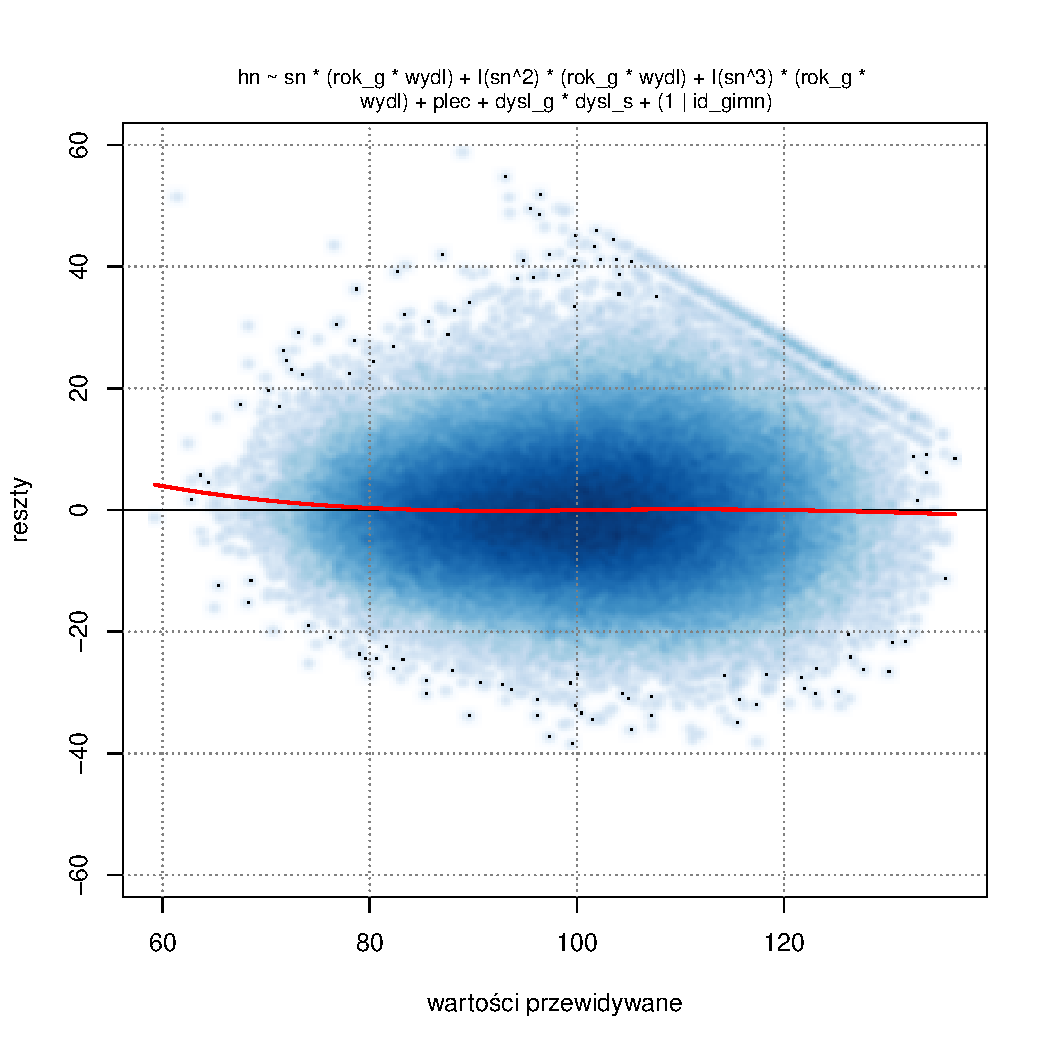
\includegraphics[width=\maxwidth]{figure/MyT11} 

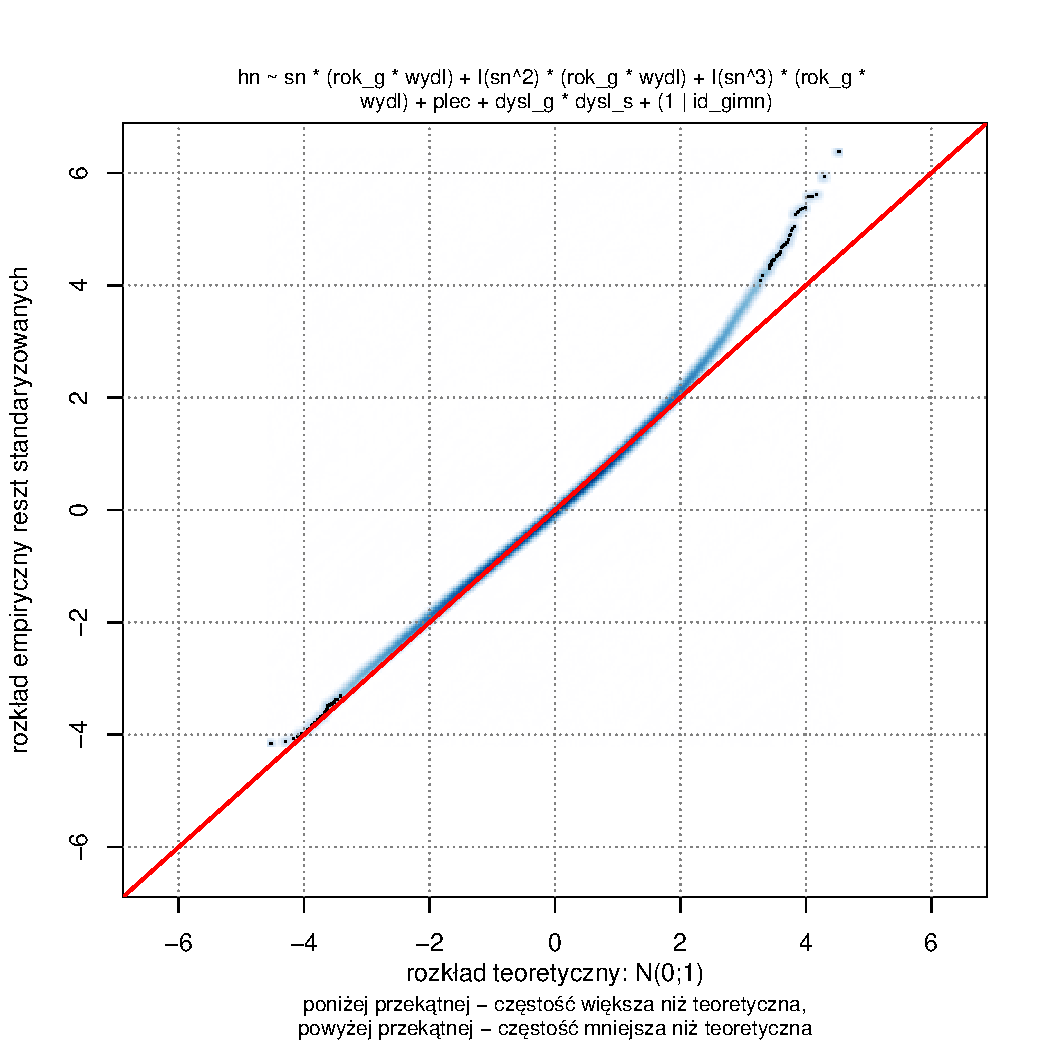
\includegraphics[width=\maxwidth]{figure/MyT12} 

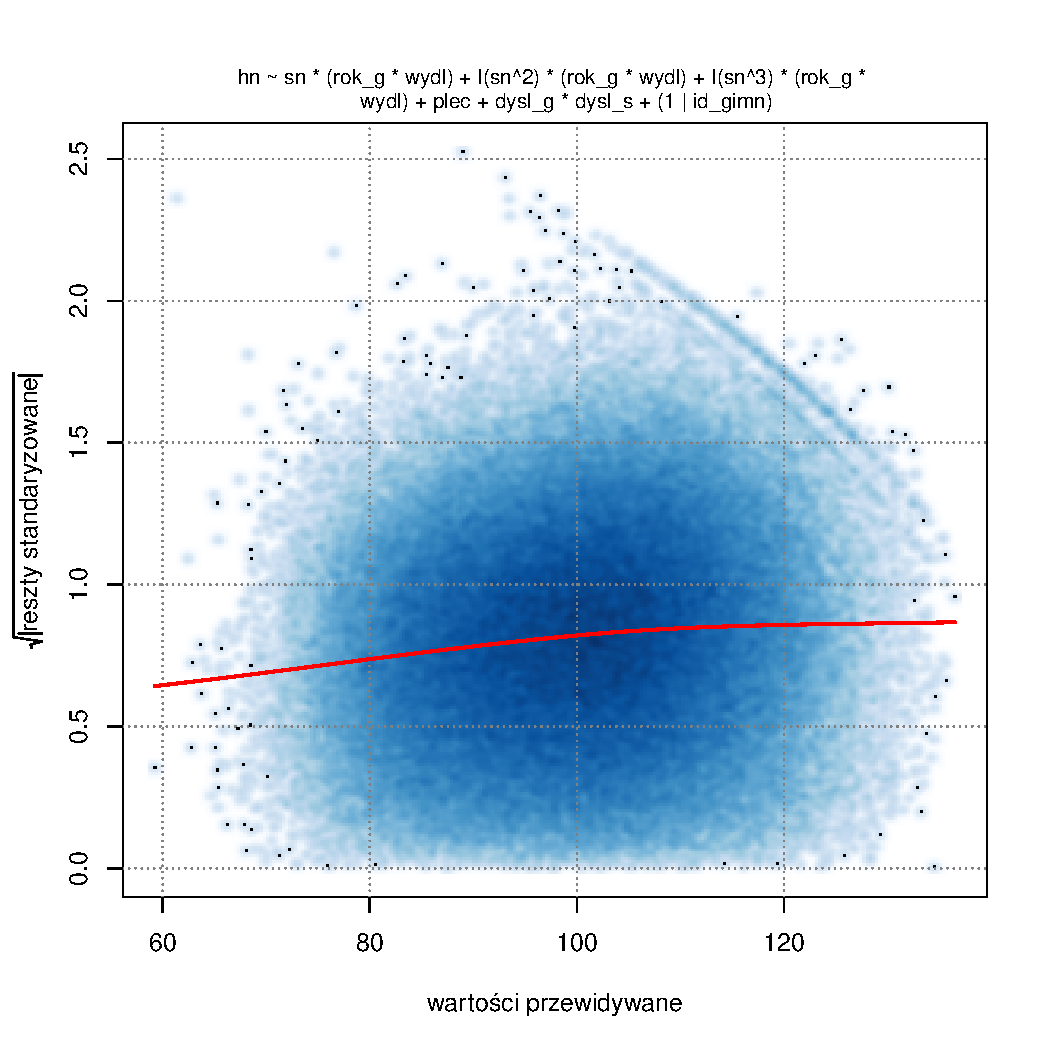
\includegraphics[width=\maxwidth]{figure/MyT13} 

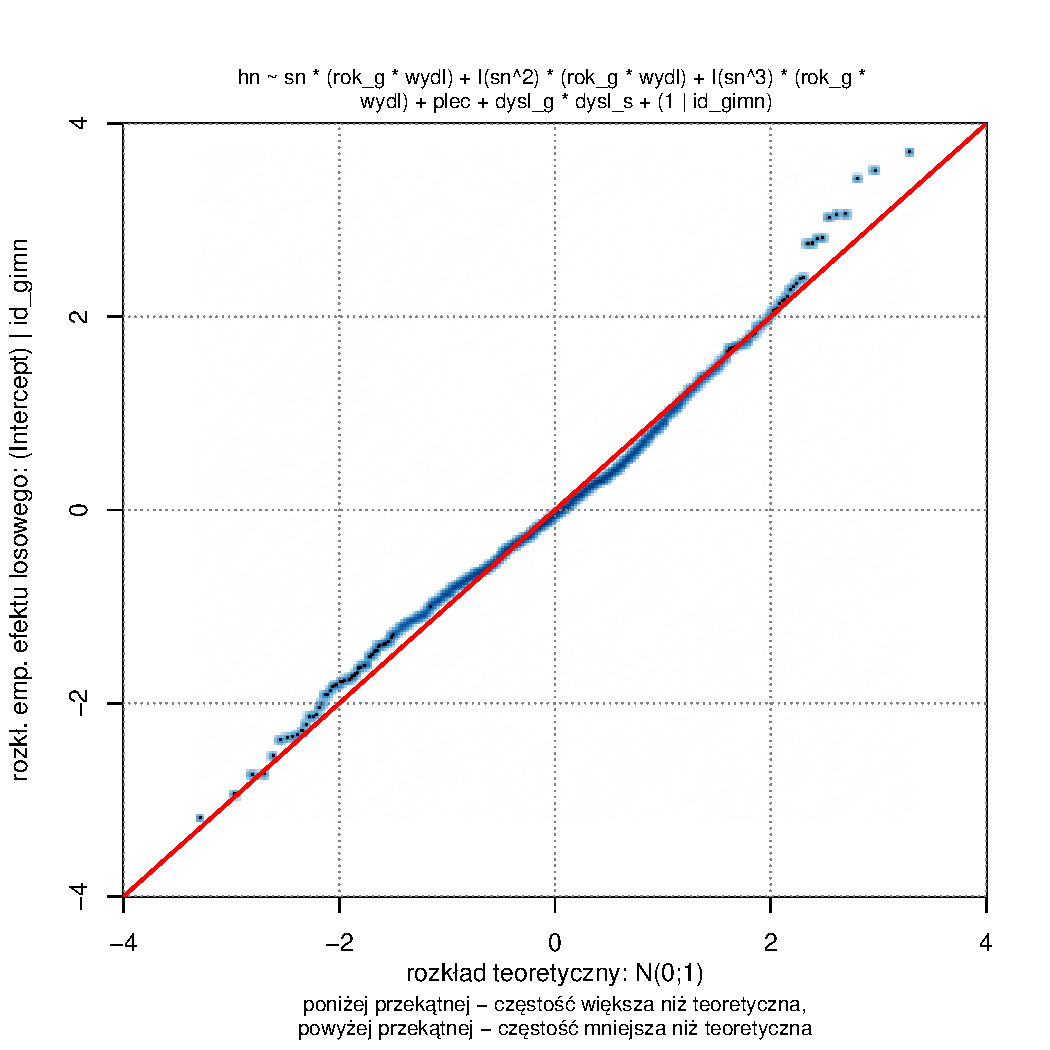
\includegraphics[width=\maxwidth]{figure/MyT14} 

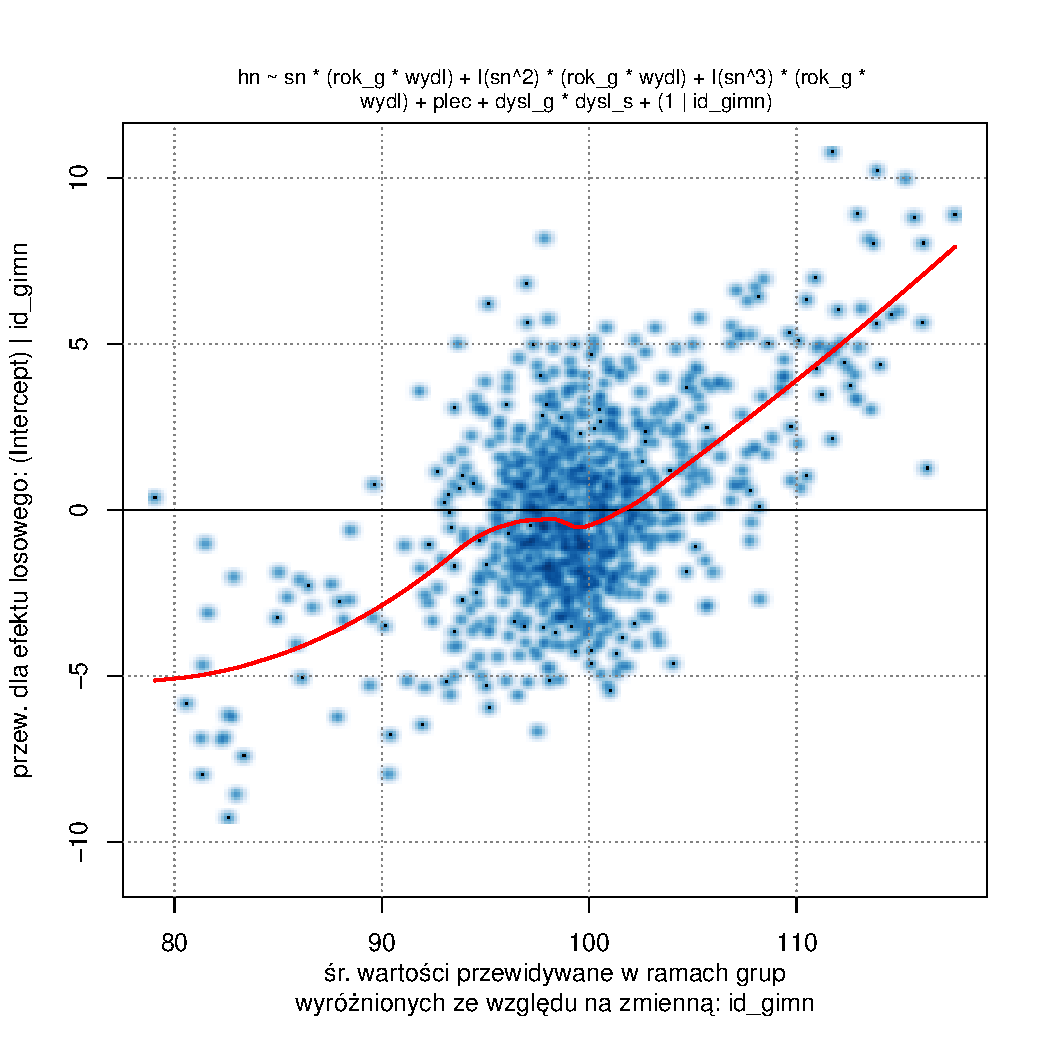
\includegraphics[width=\maxwidth]{figure/MyT15} 

\end{knitrout}
\end{comment}


\begin{document}

 
% Booktabs require to add \usepackage{booktabs} to your document preamble 
\begin{table}[tb] 
\customtitle{ Tabela 1. }{ To jest testowa tabela.} 
\begin{tabularx}{\textwidth}{@{\hspace{1.7 mm}}Xccccccc@{\hspace{1.7 mm}}} 
\midrule 
   param & Estimate & Std. Error & t value \\ \bottomrule 
   (Intercept) & 509.5426 & 72.1417 & 7.0631 \\ 
   sn & -804.8863 & 103.716 & -7.7605 \\ 
   rok\_g & -0.203 & 0.0359 & -5.6618 \\ 
   wydl & 1347.6498 & 644.9372 & 2.0896 \\ 
   I(sn\^{ }2) & -304.4479 & 48.8102 & -6.2374 \\ 
   I(sn\^{ }3) & 184.2622 & 35.2113 & 5.233 \\ 
   plecm & -1.8174 & 0.0459 & -39.567 \\ 
   dysl\_gt & 1.8008 & 0.1272 & 14.1583 \\ 
   dysl\_st & -4.492 & 0.1727 & -26.0114 \\ 
   rok\_g:wydl & -0.6731 & 0.3205 & -2.1 \\ 
   sn:rok\_g & 0.4058 & 0.0515 & 7.8723 \\ 
   sn:wydl & 3058.686 & 885.8884 & 3.4527 \\ 
   rok\_g:I(sn\^{ }2) & 0.1513 & 0.0243 & 6.2348 \\ 
   wydl:I(sn\^{ }2) & 322.9963 & 926.6895 & 0.3485 \\ 
   rok\_g:I(sn\^{ }3) & -0.0917 & 0.0175 & -5.2415 \\ 
   wydl:I(sn\^{ }3) & -238.287 & 332.0043 & -0.7177 \\ 
   dysl\_gt:dysl\_st & 0.6341 & 0.2276 & 2.7864 \\ 
   sn:rok\_g:wydl & -1.5219 & 0.4403 & -3.4563 \\ 
   rok\_g:wydl:I(sn\^{ }2) & -0.1606 & 0.4606 & -0.3486 \\ 
   rok\_g:wydl:I(sn\^{ }3) & 0.1185 & 0.165 & 0.7179 \\ 
\end{tabularx} 
\caption*{ To jest \emph{testowy} podpis. } 
\end{table} 
 
\begin{figure} 
\customtitle{Rysunek 1.}{Opis rysunku.} 
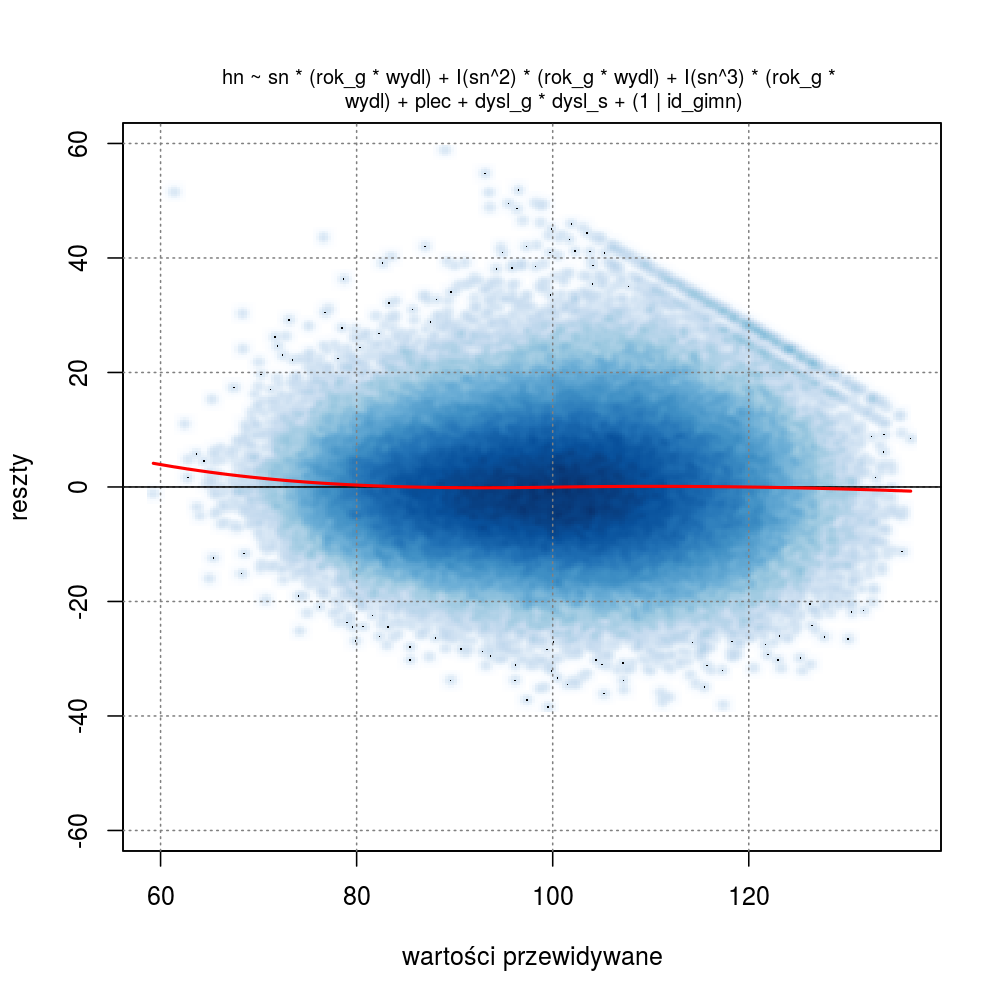
\includegraphics[width=\textwidth]{/home/grzesiek/EWDgit/EWDraport/KnitrEx/Wykresy/_reszty_w_funkcji_przewidywania.png} 
\caption*{Przypis rysunku.} 
\end{figure} 
 
% Booktabs require to add \usepackage{booktabs} to your document preamble 
\begin{table}[tb] 
\customtitle{ \textbf{Testowa} numeracja. }{ To jest testowa tabela z wykresami.} 
\begin{tabularx}{\textwidth}{@{\hspace{1.7 mm}}Xccccccc@{\hspace{1.7 mm}}} 
\midrule 
   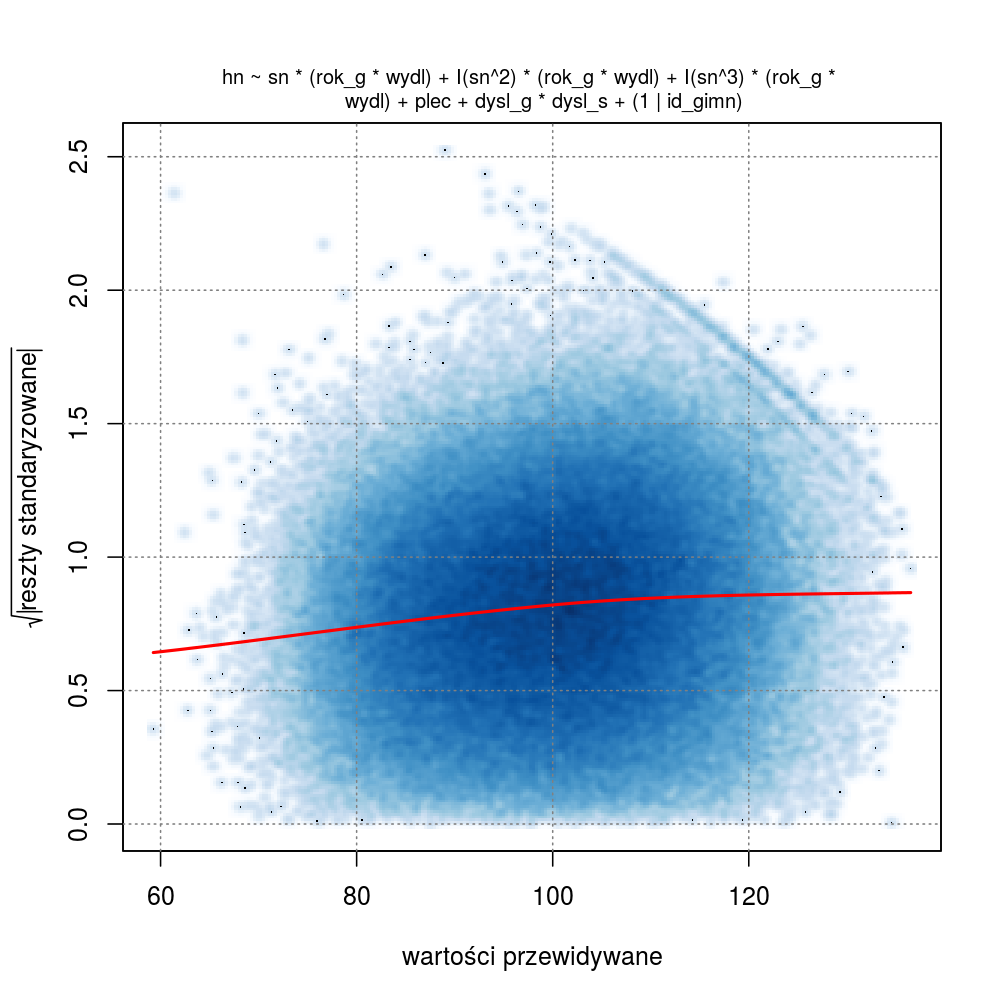
\includegraphics[width=\textwidth/2]{/home/grzesiek/EWDgit/EWDraport/KnitrEx/Wykresy/_homoscedatycznosc.png} & 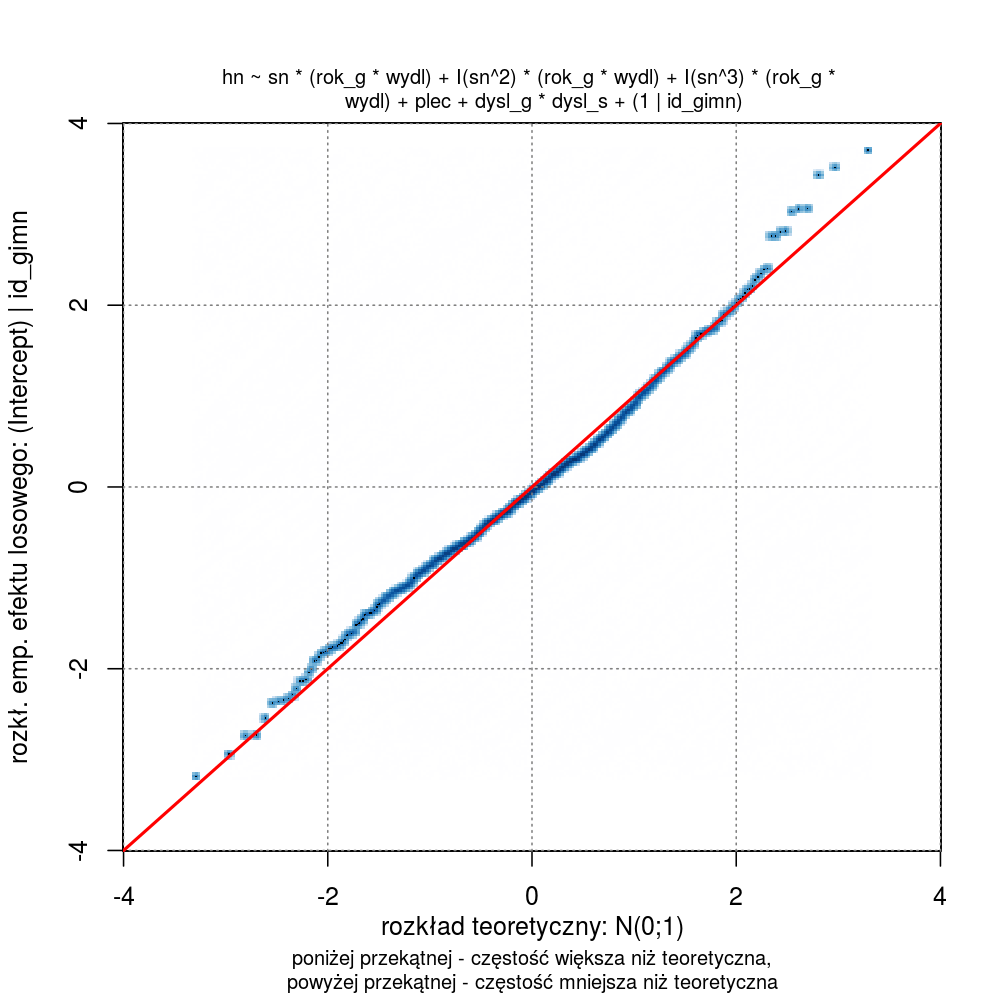
\includegraphics[width=\textwidth/2]{/home/grzesiek/EWDgit/EWDraport/KnitrEx/Wykresy/_normalnosc_ef_los_1_1.png} \\ 
   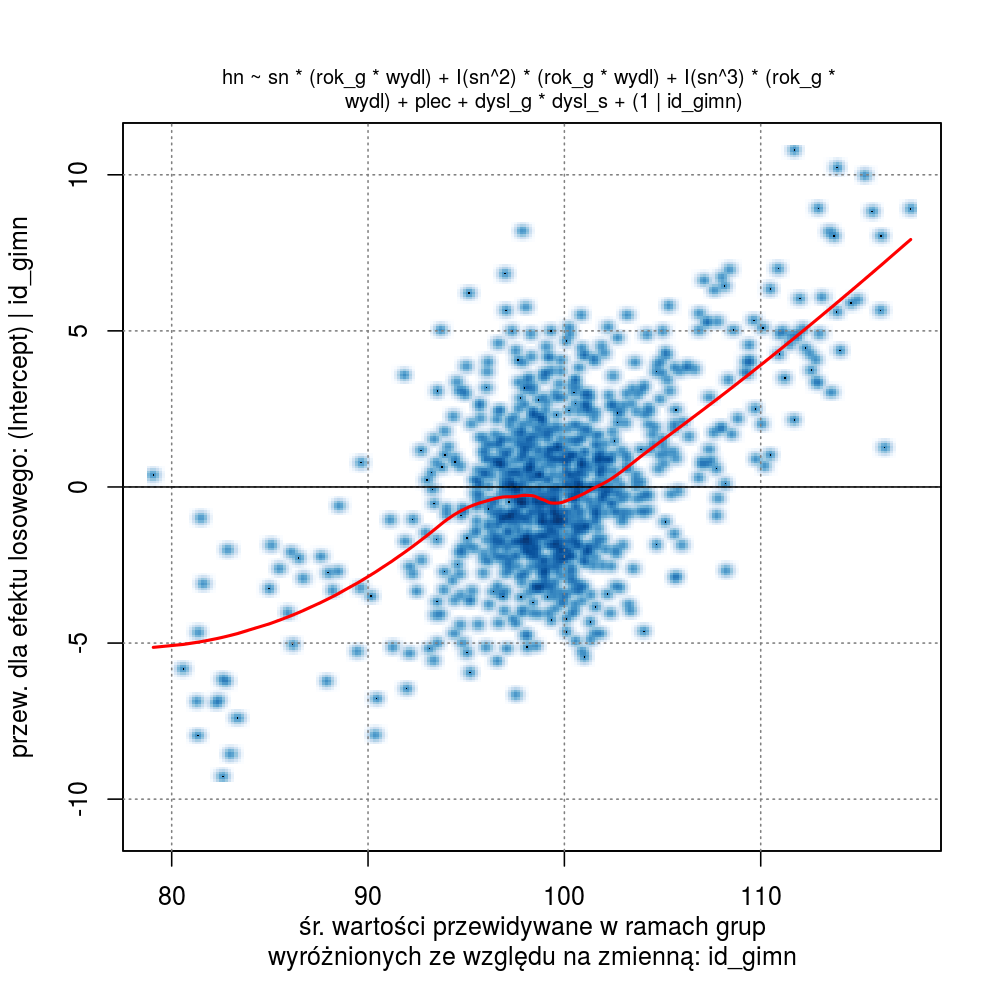
\includegraphics[width=\textwidth/2]{/home/grzesiek/EWDgit/EWDraport/KnitrEx/Wykresy/_przew_ef_los_w_funkcji_przewidywania1_1.png} & 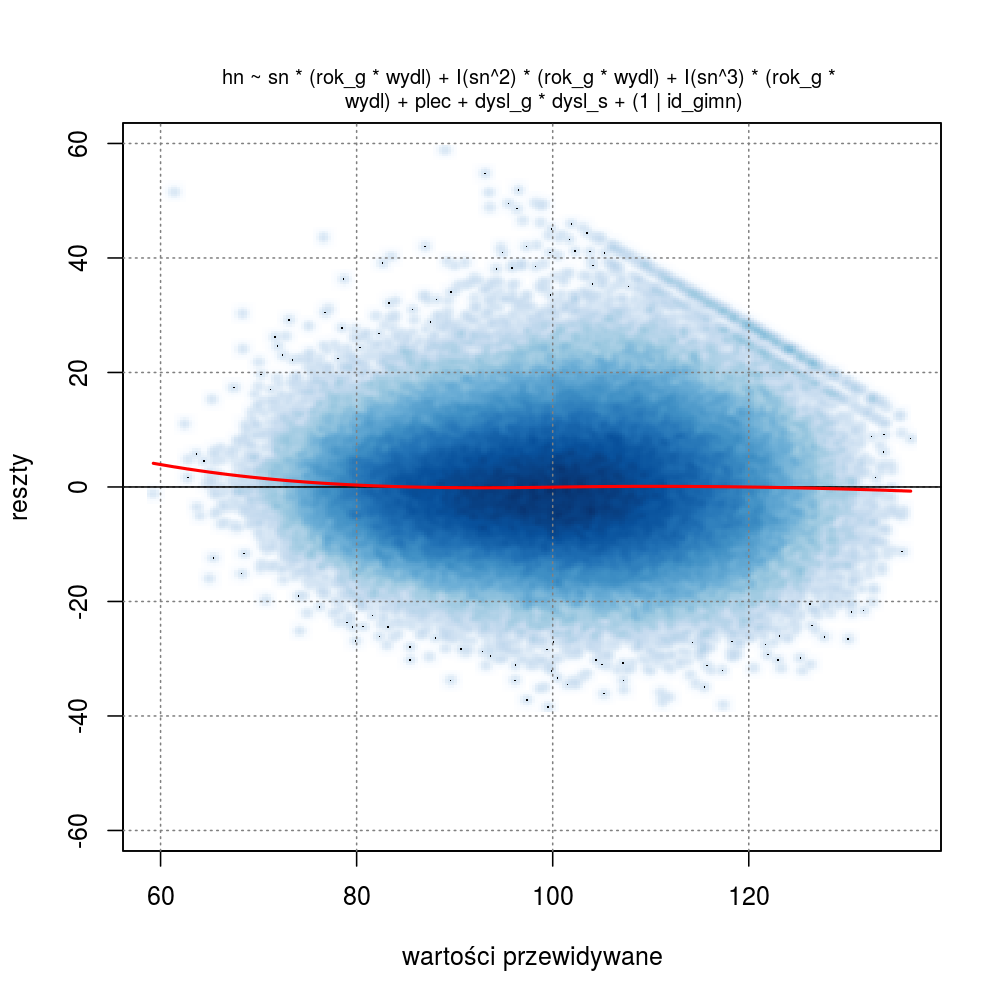
\includegraphics[width=\textwidth/2]{/home/grzesiek/EWDgit/EWDraport/KnitrEx/Wykresy/_reszty_w_funkcji_przewidywania.png} \\ 
\end{tabularx} 
\caption*{ To jest \emph{podpis} do testowej tabeli z wykresami. } 
\end{table} 
 


\end{document}
